\documentclass[10pt]{beamer}
%\usetheme{Ilmenau}
\usetheme{PaloAlto}
\usepackage[utf8]{inputenc}

\usepackage{caption}
\usepackage{graphicx}
\usepackage{amsmath}
\usepackage{amssymb}

\title{Mass Spring Damper}
\subtitle{AE 663 Project}
\institute{Indian Institute of Technology Bombay}
\author{M Suriya Kumar}
\date{\today}

\begin{document}

\begin{frame}[plain]
\maketitle
\end{frame}

\begin{frame}
\frametitle{Table of Contents}
\tableofcontents 
\end{frame}

\section{About the system}

\begin{frame}
\frametitle{Spring mass model with linear viscous damping}
\textbf{Linear viscous damping :} Linear damping occurs when a oscillatory variable is damped 
by an influence that opposes changes in it, in direct proportion to the instantaneous rate of change 
of the variable itself.

\begin{figure}[h]
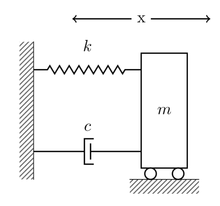
\includegraphics[scale=0.5]{spring_mass_damper.png}
\caption{Mass attached to a spring and damper}
\centering
\end{figure}

Mass($m$) is attached to a Hook's law spring and linear viscous damper. Say the spring constant 
is $k$ and damping coefficient of the damper is $c$.
\end{frame}

\begin{frame}
\frametitle{Deriving equation of motion}
From Newton's law, 
\begin{eqnarray*}
\sum f_{ext} &=& ma, \\
\sum f_{ext} &=& f_s + f_d, \\
f_s &=& -kx, 	\\
f_d &=& -c\dot{x}, \\
-kx - c\dot{x} &=& ma, \\
ma + c\dot{x} + kx &=& 0, \\
m\ddot{x} + c\dot{x} + kx &=& 0
\end{eqnarray*}

Therefore the equation of motion is given by :
\begin{equation}
m\frac{d^2x}{dt^2} + c\frac{dx}{dt} + kx = 0
\label{eom}
\end{equation}
\end{frame}


\section{Mass spring damper as generalized second order system}

\begin{frame}
\frametitle{Second order system}
General second-order system is given by :
\begin{equation}
\ddot{x} + 2\zeta\omega_0\dot{x} + \omega_0^2x = 0
\label{sec_ord_system}
\end{equation}
where $\zeta$ is called damping ratio and $\omega_0$ is called natural frequency.
From \ref{eom} we can get,
\begin{equation}
\ddot{x} + \frac{c}{m}\dot{x} + \frac{k}{m}x = 0
\label{mass_spring_system}
\end{equation}

Comparing coefficient with \ref{sec_ord_system}, we get
\begin{eqnarray}
\zeta &=& \frac{c}{2\sqrt{km}}, \\
\label{def_zeta}
\omega &=& \sqrt{\frac{k}{m}}
\label{def_omega}
\end{eqnarray}

\end{frame}

\section{Types of responses}

\begin{frame}
\frametitle{Types of responses}
\begin{itemize}
	\item{Free response}\\
	In free response the external force is 0. That is the equation of 
	motion is given by :
	$$ \ddot{x} + \frac{c}{m}\dot{x} + \frac{k}{m}x = 0 $$

	\item{Forced dynamic response}\\
	In forced response there exist a external force apart from spring force and 
	viscous damping force. That is the equation of motion is given by :
	$$ \ddot{x} + \frac{c}{m}\dot{x} + \frac{k}{m}x = F(\dot{x},x,t) $$

\end{itemize}

\end{frame}


\section{State space model of the system}

\begin{frame}
\frametitle{State space model of the system}
We can describe the system only by its position and velocity. Therefore the state-space model
of the system is given by :

\end{frame}

\section{Classification}

\begin{frame}
\frametitle{Classification of system based on damping ratio}
\begin{itemize}
	\item{Under-damped system ($\zeta < 1$)}
	\item{Critically damped system ($\zeta = 1$)}
	\item{Over-damped system ($\zeta > 1$)}
\end{itemize}
\end{frame}

\begin{frame}
\frametitle{Under-damped system}
In under-damped system $\zeta$ is less than 1.
The free response of the system is shown in the figure below$\phantom{}_{\ref{fig1}}$.

\begin{figure}[h]
	\centering
	\includegraphics[width=0.8\textwidth, height=0.7\textheight]{Free_response_underdamped.png}
	\caption{Free response of a spring mass damper system}
\end{figure}
\label{fig1}

\end{frame}


\begin{frame}
The forced response of the system is shown in the figure below$\phantom{}_{\ref{fig2}}$.

\begin{figure}[h]
	\begin{tabular} {l c}
	\includegraphics[width=0.45\textwidth, height=0.5\textheight]{Forced_response_underdamped_under.png} &
	\includegraphics[width=0.45\textwidth, height=0.5\textheight]{Forced_response_underdamped_over.png} 
	\end{tabular}
	\caption{Forced response of a spring mass damper system}
\end{figure}
\label{fig2}

\end{frame}
 
\begin{frame}
The forced response of the system is shown in the figure below$\phantom{}_{\ref{fig3}}$.

\begin{figure}[h]
	\begin{tabular} {l}
	\includegraphics[width=0.8\textwidth, height=0.7\textheight]{Forced_response_underdamped_natural.png} 
	\end{tabular}
	\caption{Forced response of a spring mass damper system}
\end{figure}
\label{fig3} 

\end{frame}

\begin{frame}
\frametitle{Over-damped system}
In under-damped system $\zeta$ is more than 1.
The free response of the system is shown in the figure below$\phantom{}_{\ref{fig4}}$.

\begin{figure}[h]
	\centering
	\includegraphics[width=0.8\textwidth, height=0.7\textheight]{Free_response_overdamped.png}
	\caption{Free response of a spring mass damper system}
\end{figure}
\label{fig4}

\end{frame}


\begin{frame}
The forced response of the system is shown in the figure below$\phantom{}_{\ref{fig5}}$.

\begin{figure}[h]
	\begin{tabular} {l c}
	\includegraphics[width=0.45\textwidth, height=0.5\textheight]{Forced_response_overdamped_under.png} &
	\includegraphics[width=0.45\textwidth, height=0.5\textheight]{Forced_response_overdamped_over.png} 
	\end{tabular}
	\caption{Forced response of a spring mass damper system}
\end{figure}
\label{fig5}

\end{frame}
 
\begin{frame}
The forced response of the system is shown in the figure below$\phantom{}_{\ref{fig6}}$.

\begin{figure}[h]
	\begin{tabular} {l}
	\includegraphics[width=0.8\textwidth, height=0.7\textheight]{Forced_response_overdamped_natural.png} 
	\end{tabular}
	\caption{Forced response of a spring mass damper system}
\end{figure}
\label{fig6} 

\end{frame}


\begin{frame}
\frametitle{Special case}
A special case of the system arises when there is zero damping i.e $c = 0$ or $\zeta$ is zero. \\
The free response of the system is shown in the figure below$\phantom{}_{\ref{fig7}}$.

\begin{figure}[h]
	\centering
	\includegraphics[width=0.7\textwidth, height=0.55\textheight]{Free_response_special.png}
	\caption{Free response of a spring mass damper system}
\end{figure}
\label{fig7}

\end{frame}


\begin{frame}
The forced response of the system is shown in the figure below$\phantom{}_{\ref{fig5}}$.

\begin{figure}[h]
	\begin{tabular} {l c}
	\includegraphics[width=0.45\textwidth, height=0.5\textheight]{Forced_response_special_under.png} &
	\includegraphics[width=0.45\textwidth, height=0.5\textheight]{Forced_response_special_over.png} 
	\end{tabular}
	\caption{Forced response of a spring mass damper system}
\end{figure}
\label{fig8}

\end{frame}
 
\begin{frame}

Upon forcing the system under natural frequency in this special case a resonance is observed. Under this
forcing the positon variable explodes as time goes to $\infty$.\\
Forced response is shown in the figure below$\phantom{}_{\ref{fig6}}$.

\begin{figure}[h]
	\begin{tabular} {l}
	\includegraphics[width=0.7\textwidth, height=0.6\textheight]{Forced_response_special_natural.png} 
	\end{tabular}
	\caption{Forced response of a spring mass damper system}
\end{figure}
\label{fig9} 

\end{frame}

\section{Dynamic response}

\begin{frame}
\frametitle{Detailed analysis of forced response}
Solving the followwing equation,
$$ m\ddot{x} + c\dot{x} + kx = F(\dot{x},x,t) $$

we get 
$$ x(t) = x_p(t) + x_h(t)$$
where $x_p(t)$ is the particular solution and $x_h(t)$ is the homogeneous solution

\end{frame}

\begin{frame}
\frametitle{Hoarmonic forcing}
Under harmonic forcing equation of motion is given by,

\begin{eqnarray}
m\ddot{x} + c\dot{x} + kx &=& F_0cos\omega t
\end{eqnarray}
Solving for particular solution, we get
\begin{eqnarray}
x_p(t) &=& Xcos(\omega t - \phi)
\end{eqnarray}
Upon substituting particular solution in equation of motion, we get

\begin{eqnarray}
X[(k - m\omega_0^2)cos\phi + c\omega sin\phi] &=& F_0, \\ 
X[(k - m\omega_0^2)sin\phi - c\omega cos\phi] &=& 0 
\end{eqnarray}

\end{frame}

\begin{frame}
Solving for $\phi$ and $X$, we get

\begin{eqnarray}
\phi &=& tan^{-1} \left( \frac{c\omega}{k - m\omega^2} \right), \\
\label{X}
X &=& \frac{F_0}{\sqrt{\left( k - m\omega^2\right)^2 - c^2\omega^2}}
\end{eqnarray}

Upon rearranging the terms in \ref{X}, we get 

\begin{eqnarray}
X &=& \frac{ \frac{F_0}{k} }{ \sqrt{ \left( 1 - \frac{\omega^2}{\omega_0^2} \right)^2 - \left( 2\zeta \frac{\omega}{\omega_0} \right)^2 } }, \\
\implies X &=& \frac{ \eta_{st} }{ \sqrt{ \left( 1 - r^2 \right)^2 + \left( 2\zeta r \right)^2 } } 
\end{eqnarray}

\end{frame}

\begin{frame}
Where,
\begin{eqnarray}
\eta_{st} &=& \frac{F_0}{k}, \\
r &=& \frac{\omega}{\omega_0}
\end{eqnarray}

$\eta_{st}$ is the maximum displacement when there is a static force $F_0$ applied. \\
The ratio  of $X$ and $\eta_{st}$ is called dynamic magnifaction factor. \\
We can see that when there is no damping, dynamic magnification factor approaches $\infty$ 
when the system is forced at natural frequency. This phenomenon is called resonance. Which means 
however small the static force($F_0$), $x$ $\rightarrow$ $\infty$ as time $\rightarrow$ $\infty$

\end{frame}

 
\end{document}

